\documentclass[twoside,a4paper]{article}
% Langage et encodage
\usepackage[english]{babel}
\usepackage[utf8]{inputenc}
\usepackage[T1]{fontenc}
\usepackage{lmodern}

% UPMC recommendations for margin sizes
\usepackage[left=2.5cm,right=2.5cm,top=1.5cm,bottom=2.0cm,includefoot,includehead,headheight=13.6pt]{geometry}
\setlength{\skip\footins}{0.7cm}
\usepackage[bottom]{footmisc}

% Tableaux
\usepackage{longtable}
\usepackage{tabularx}
\usepackage{multirow}
\usepackage{booktabs}
%\addto\captionsfrench{\def\tablename{Table}}

% Typo et formules
\usepackage{eurosym} % Symbole euro
\usepackage{latexsym} % Additional symbols
\usepackage{url} % citer des adresses électroniques et des URL
\usepackage{amsmath,amssymb,amsthm} % AMS Math
\usepackage{leftidx} % Better sub and superscripts
\usepackage[mediumspace,mediumqspace,Grey,squaren]{SIunits} % SI units

% Biblio
\usepackage{natbib} % Package for multiple citation with author-date style
%\setcitestyle{citesep={~;}} % Semicolon separator with french typography
\usepackage{microtype}
\usepackage{breakcites}
\usepackage[hyphenbreaks]{breakurl}
\def\UrlBreaks{\do\/\do-}


% Puces numérotées
\usepackage{enumitem}
\setlist{noitemsep}

% Figures
\usepackage{graphicx}
\usepackage{subfigure}
\usepackage{rotating} % Sideways of figures & tables
\usepackage[singlelinecheck=false]{caption} % Package for caption

%\DeclareCaptionLabelSeparator{virg}{~: } % New caption label separator
%\captionsetup{labelfont=bf,textfont=it,labelsep=virg} % Set fonts and label separators
%\addto\captionsfrench{%
%  \renewcommand{\listfigurename}{Liste des figures}%
%}

%% Table of contents for each chapter
%\usepackage{tocbibind}
%\usepackage[french]{minitoc}
%\setcounter{minitocdepth}{2}
%\mtcindent=15pt
%\renewcommand{\mtcSfont}{\small\normalfont} % Normal font for minitoc entries
%\newcommand{\miniminitoc}{\minitoc \vspace{12pt}}
%% Use \dominitoc at the beginning of the document
%% Use \minitoc where to put a table of contents

% Nicer backref links
\usepackage[breaklinks=true,bookmarks=true,pagebackref,hyperindex=true,pdfa]{hyperref}
\backreffrench
\renewcommand*{\backref}[1]{}
\renewcommand*{\backrefalt}[4]{%
\ifcase #1 %
(Non cited)%
\or
(Cited page~#2)%
\else
(Cited pages~#2)%
\fi}
\renewcommand*{\backrefsep}{, }
\renewcommand*{\backreftwosep}{ and~}
\renewcommand*{\backreflastsep}{ and~}

% Informations included in the pdf file
\hypersetup
{
bookmarksopen=true,
pdftitle="Surface-Wave dispersion Inversion and Profiling",
pdfauthor="Sylvain PASQUET", %auteur du document
pdftoolbar=false, %barre d'outils non visible
pdfmenubar=true, %barre de menu visible
pdfhighlight=/O, %effet d'un clic sur un lien hypertexte
colorlinks=true, %couleurs sur les liens hypertextes
pdfpagemode=UseNone, %aucun mode de page
pdfpagelayout=SinglePage, %ouverture en simple page
pdffitwindow=true, %pages ouvertes entierement dans toute la fenetre
linkcolor=black, %couleur des liens hypertextes internes
citecolor=blue, %couleur des liens pour les citations
urlcolor=black, %couleur des liens pour les url
hyperfootnotes=true
}


\frenchspacing\sloppy
\def\labelitemi{--}

\title{\Huge{\textbf{SWIP User's Manual}}}
\author{\Large{Sylvain Pasquet} (\url{spasquet@uwyo.edu})}

\date{\LARGE{Version 1.0: May 2016}\\
\vspace{2.5cm}
\large{The Surface-Wave dispersion Inversion and Profiling software is supported by:\\
\vspace{1.5cm}
\textbf{University of Wyoming}\\
Department of Geology and Geophysics\\
Wyoming Center for Environmental Hydrology and Geophysics\\
\bigskip

\includegraphics[scale=0.04]{./figures/logo_UW_brown_2L.png}
\hspace{0.5cm}

\includegraphics[scale=0.05]{./figures/logo_dept_geol_geophy.png}
\hspace{0.5cm}

\includegraphics[scale=0.21]{./figures/logo_WyCEHG.png}\\
\bigskip
Laramie, WY 82070, USA\\
\vspace{1.5cm}
\textbf{Université Pierre et Marie Curie}\\
UMR 7619 METIS\\
\bigskip

\includegraphics[scale=0.095]{./figures/logo_upmc.png}
\hspace{0.5cm}

\includegraphics[scale=0.125]{./figures/logo_metis.png}\\
\bigskip
75005 Paris, France}}


\begin{document}
\maketitle
\thispagestyle{empty}
\newpage
\tableofcontents

\newpage
\section{Installation instructions}
SWIP is a MATLAB-based software originally developped to work under a GNU/Linux distribution. It executes binaries from the open software packages \textbf{Seismic Unix} and \textbf{Geopsy}. It (optionally) requires the open software packages \textbf{ImageMagick}, \textbf{PDFjam}, and \textbf{pdfcrop}.

\bigskip\noindent
To work under Windows, you need to install the Linux-like environment \textbf{Cygwin} in order to run \textbf{Seismic Unix} binaries.

\bigskip\noindent
Whatever OS you are using, you will need the administrator/root rights to install SWIP.

\subsection{First steps}
\begin{itemize}
\setlength\itemsep{2ex}
\setlength{\parindent}{5ex}
\item Get the latest version of the code available at \url{https://github.com/SWIPdev/SWIP/releases}. Download the zipped file \verb|SWIP-x.x.zip| or the gzipped tarfile \verb|SWIP-x.x.tar.gz| containing the source codes for SWIP (the "x.x" is the current Release number).

\item If not already installed, install MATLAB on your computer (no extra toolbox is required). A change of graphics engine in MATLAB 2014b and higher causes problem with figures output (slow figure display, huge output file size). To avoid those problems, I recommend to use an older version of MATLAB.\\[1ex]
To download an older version, you need to create a Mathworks account (\url{http://www.mathworks.com}) and download the selected release (\url{http://fr.mathworks.com/downloads/select_release?mode=gwylf}). If you are using a network license, just create an account using your institution email. For a standalone license, you will need to associate it with your Mathworks account in the License Center (\textit{Associate License} on the top right of the screen). When installing MATLAB, you will just need to login to your Mathworks account and provide the path of the license file to activate it.

\item Once MATLAB is installed, you will need to extract the content of the SWIP archive file in your MATLAB path (refered later as \verb|/your/MATLAB/path|) and give MATLAB access to the contents of this folder. To decompress the file, use the command \verb|tar -xzf SWIP_xx.tar.gz| in the terminal if you are under Linux, or use a software like 7zip if you are under Windows. In MATLAB, go in \textit{File->Set Path->Add with Subfolders} to select the \verb|SWIP| folder, then \textit{Save} and \textit{Close}.\\[1ex]
Examples of \verb|/your/MATLAB/path| directory:

\verb|/home/yourusername/Documents/MATLAB| under GNU/Linux distributions

\verb|C:\Users\yourusername\Documents\MATLAB| under Windows distributions\\[1ex]
Type \verb|swip_version| in the MATLAB prompt to check if the scripts are correctly installed.
\end{itemize}

\subsection{Install on GNU/Linux}
I only tested SWIP with a standard Ubuntu distribution, but the procedure should be similar for MacOS and other GNU/Linux distributions.
\subsubsection{Prerequisites}
Before installing Seismic Unix and/or Geopsy, you need to make sure that these libraries and packages are installed on your computer:

\begin{itemize}
\item \verb|gcc|
\item \verb|gfortran|
\item \verb|qt4-qmake|
\item \verb|libqt4-dev|
\item \verb|liblapack-dev|
\item \verb|libfftw3-dev|
\item \verb|zlib1g-dev|

\end{itemize}
\subsubsection{Seismic Unix}
\textit{The installation of Seismic Unix is only necessary to handle seismic data in order to compute, stack and pick dispersion images. If you have your own software for picking dispersion curves and just want to use SWIP to invert them, you can skip the installation of SU.}\\[2ex]
The following instructions are mainly copied from the Seismic Unix (SU) \verb|Installation_Instructions| file (\url{http://www.cwp.mines.edu/cwpcodes/Installation_Instructions}). Refer to it for more detailed instructions.

\begin{itemize}
\setlength\itemsep{2ex}
\setlength{\parindent}{5ex}
\item Download SU at \url{http://www.cwp.mines.edu/cwpcodes}

\item Create a directory that will contain all the SU codes (refered later as \verb|/your/SU/path|). This directory should be owned by you (meaning you have write/read/execute rights) and located in a partition with at least 100 Mb available.\\[1ex]
Examples of \verb|/your/SU/path| directory:

\verb|/usr/local/SU|

\verb|/home/yourusername/SU|

\verb|/opt/SU|

\item Decompress the gzipped tarfile \verb|cwp_su_all_xx.tgz| (the "xx" is the current Release number) in \verb|/your/SU/path|, the directory \verb|/your/SU/path/src| will appear, containing all of the source code. To decompress the file, use the command \verb|tar -xzf cwp_su_all_xx.tgz| in the terminal.


\item Set the necessary environment variable and the binaries path. Open the file \verb|.profile| located in \verb|/home/yourusername| with a text editor (e.g. \verb|gedit|) (type \verb|ls -la| in the terminal to see it) and add the following lines at the end of the file:

\verb|export CWPROOT=/your/SU/path|

\verb|PATH=$PATH:/your/SU/path/bin|

\verb|export PATH|\\[1ex]
Relog your session and check if these are correctly set by typing \verb|echo $CWPROOT| and \verb|echo $PATH| in the terminal.

\item In the \verb|/your/SU/path/src/configs| directory, select the file \verb|Makefile.config_your_system| corresponding to your configuration, rename it \verb|Makefile.config| and copy it in \verb|/your/SU/path/src| to replace the existing \verb|Makefile.config|.

\item In the terminal, go in the \verb|/your/SU/path/src| directory by typing \verb|cd /your/SU/path/src|. You will then compile the codes by typing:

\verb|make install| => install the basic SU codes

\verb|make xtinstall| => install the X windows codes (not necessary for SWIP)

\verb|make xminstall| => install the Motif based codes (not necessary for SWIP)\\[1ex]
If you have to recompile along the way, type:

\verb|make remake| => recompile the basic SU codes

\verb|make xtinstall| => recompile the X windows based codes (not necessary for SWIP)

\verb|make xminstall| to recompile the Motif based codes (not necessary for SWIP)

\item Type the command \verb|sukeyword -o| in the terminal to check if SU is correctly installed.
\end{itemize}

\subsubsection{SU extra binaries}
Two extra codes, non-available in the default SU release, are required to run SWIP. The first one, \verb|supomegal|, computes the $p-\omega$ transform of a seismogram in the $x-t$ domain in order to retrieve a dispersion image in the $v-f$ domain. The second one, \verb|seg2segy|\footnote{\textbf{seg2segy} is available as a third party in SU, but does not work correctly on 64 bits systems. The version provided here has been modified to work under 64 bits environments.}, allow to convert SEG2 files usually obtained on the field in SEGY files which can then be converted in the SU files required to use SWIP (for more details, see section \ref{sec:seg2su}).\\[1ex]
To install these codes, follow these steps in the terminal:
\begin{itemize}
\setlength\itemsep{2ex}
\setlength{\parindent}{5ex}
\item Go in the \verb|SWIP/src| directory by typing:

\verb|cd /your/MATLAB/path/SWIP/src|

\item Assign "execute" permission to the \verb|configure| file by typing:

\verb|chmod +x configure|

\item Compile and install the codes by typing:

\verb|./configure|

\item Type the commands \verb|supomegal| and \verb|seg2segy| in the terminal to check if they are correctly installed.

\end{itemize}

\subsubsection{Geopsy}
For more information about installing Geopsy under Linux, please refer to the Geopsy webpage (\url{http://www.geopsy.org/wiki/index.php/Installation:Linux}).
\begin{itemize}
\setlength\itemsep{2ex}
\setlength{\parindent}{5ex}
\item Download the Linux version of Geopsy at \url{http://www.geopsy.org/download.php}.

\item Create a directory that will contain all the Geopsy codes (refered later as \verb|/your/Geopsy/path|). This directory should be owned by you (meaning you have write/read/execute rights) and located in a partition with at least 30 Mb available.\\[1ex]
Examples of \verb|/your/Geopsy/path| directory:

\verb|/usr/local/Geopsy.org| (default)

\verb|/home/yourusername/Geopsy.org|

\verb|/opt/Geopsy.org|

\item Decompress the gzipped tarfile \verb|geopsypack-nnitems-src-xx.tgz| ("nn" is the number of items and "xx" is the current Release number) in \verb|/your/Geopsy/path|, the directory \verb|/your/SU/path/geopsypack-nnitems-src-xx| will appear, containing all of the source code. To decompress the file, use the command \verb|tar -xzf geopsypack-nnitems-src-xx.tgz| in the terminal.

\item Set the binaries path in the file \verb|.profile| located in \verb|/home/yourusername| with a text editor (e.g. \verb|gedit|) (type \verb|ls -la| in the terminal to see it) and extend the \verb|PATH| line (see SU installation) with \verb|:/your/Geopsy/path/bin| such as:

\verb|PATH=$PATH:/your/SU/path/bin:/your/Geopsy/path/bin|\\[1ex]
Relog your session and check if the path is correctly set by typing \verb|echo $PATH| in the terminal.

\item In the terminal, go in the \verb|/your/SU/path/geopsypack-nnitems-src-xx| directory by typing \verb|cd /your/SU/path/geopsypack-nnitems-src-xx|.\\[1ex]
To configure the installation in the default \verb|/your/Geopsy/path| directory, type:

\verb|./configure|\\[1ex]
To configure the installation in a custom \verb|/your/Geopsy/path| directory, type:

\verb|./configure -prefix /your/Geopsy/path|

\item You will then compile the codes by typing:

\verb|make install|
\end{itemize}

\subsubsection{Additionnal packages}
Some additionnal packages can be installed to concatenate figure results and produce publication ready final figures (otherwise SWIP produces separate figures). ImageMagick is used to crop and concatenate raster (PNG, JPEG,...) images in order to create figure panels ready for publicactions. PDFcrop cuts the extra edges around PDF created by MATLAB, while PDFjam is used to concatenate PDF images.
\begin{itemize}
\setlength\itemsep{2ex}
\item Install ImageMagick by typing in the terminal: \verb|sudo apt-get install imagemagick|
\item Install PDFjam by typing in the terminal: \verb|sudo apt-get install pdfjam|
\item Install pdfcrop by typing in the terminal: \verb|sudo apt-get install texlive-extra-utils|
\end{itemize}

\subsubsection{Known problems}
\begin{itemize}
\setlength\itemsep{2ex}
\setlength{\parindent}{5ex}
\item When starting MATLAB (version < 2011b), the error message \textit{Error while loading shared library libXp.so.6} can appear. A workaround can be found here:

\url{http://fr.mathworks.com/matlabcentral/answers/99815-why-do-i-receive-xsetup-errors-regarding-libxp-so-6-when-installing-or-launching-matlab-on-fedora-co}

\item When running the inversion (module C, with verbose=1), MATLAB can give you the error message \textit{dinver: symbol lookup error: /opt/Geopsy.org/lib/libQGpGuiTools.so.1: undefined symbol: \_ZN12QApplication10commitDataER15QSessionManager}.\\[1ex]
It means there is a conflict between Ubuntu QT libraries and MATLAB QT libaries. A workaround is to delete the redundant libraries of MATLAB. These libraries are usually found in:

\verb|/your/MATLAB/path/bin/glnxa64/libQtGui.so.4|

\verb|/your/MATLAB/path/bin/glnxa64/libQtNetwork.so.4|

\verb|/your/MATLAB/path/bin/glnxa64/libQtCore.so.4|
\end{itemize}

\subsection{Install on Windows}
SWIP has been successfully installed on Windows 7 and Windows 10. The procedure should be very similar on other Windows versions. As mentionned earlier, the Linux-like environment Cygwin is currently required to run Seismic Unix on Windows. However, Microsoft has just announced that Windows 10 will soon be able to run Bash and compile Linux binaries with the Windows Subsystem for Linux (\url{https://msdn.microsoft.com/en-us/commandline/wsl/about}). Hopefully we will soon be able to run Seismic Unix without any third party software like Cygwin.

\subsubsection{Cygwin}
\textit{The installation of Cygwin is only necessary to run Seismic Unix (see \ref{subsec:WinSU}). and ImageMagick (see \ref{subsec:WinExtra}). If you don't need SU or ImageMagick, you can skip the installation of Cygwin.}
\begin{itemize}
\setlength\itemsep{2ex}
\setlength{\parindent}{5ex}
\item Download the 32 bits version of Cygwin available at \url{http://www.cygwin.com/setup-x86.exe} (I could not install SU with the 64 bits version, but if you want to give it a try, be my guest and let me know).

\item Run \verb|setup-x86.exe|. When asked, choose \textit{Install from Internet}. Select the root directory to install Cygwin (refered later as \verb|\your\cygwin\path|). Make sure it is located in a partition with at least 1 Gb available. Finally, select any of the proposed mirrors to download the data.
Examples of \verb|\your\cygwin\path| directory:

\verb|C:\cygwin| (default)

\verb|C:\Program Files\cygwin|

\item Keep the default install, and add the following packages (use the search bar to find them, then click once on the circle arrow to select them):

\verb|make gcc-core gcc-fortran gcc-g++| in \textit{Devel}

\verb|libgcc1 libgfortran3 libmcpp-devel libmcpp0| in \textit{Libs}

\verb|ImageMagick| in \textit{Graphics}

\item Once all the required packages are selected, click Next (keep "select required packages" checked) to start the installation.

\item If you want to use the graphics capabilities of Seismic Unix, you need to install the X11 libraries in Cygwin.
\end{itemize}

\subsubsection{Seismic Unix}
\label{subsec:WinSU}
\textit{The installation of Seismic Unix is only necessary to handle seismic data in order to compute, stack and pick dispersion images. If you have your own software for picking dispersion curves and just want to use SWIP to invert them, you can skip the installation of SU.}\\[2ex]
The following instructions are mainly copied from the Seismic Unix (SU) \verb|Installation_Instructions| file (\url{http://www.cwp.mines.edu/cwpcodes/Installation_Instructions}).
\begin{itemize}
\setlength\itemsep{2ex}
\setlength{\parindent}{5ex}
\item Download Seismic Unix at \url{http://www.cwp.mines.edu/cwpcodes}

\item Create a directory that will contain all the SU codes (refered later as \verb|/your/SU\path|). This directory should be owned by you (meaning you have write/read/execute rights) and located in a partition with at least 100 Mb available. I recommend that you create \verb|/your/SU/path| in the root folder of Cygwin \verb|\your\cygwin\path|.\\[1ex]
Examples of \verb|/your/SU/path| directory (assuming that you create it from the Cygwin terminal in the root folder of Cygwin):

\verb|/home/yourusername/SU|

\verb|/usr/local/SU|

\verb|/opt/SU|\\[1ex]
In the Windows Explorer, this directory will look like:

\verb|C:\cygwin\home\yourusername\SU|

\verb|C:\cygwin\usr\local\SU|

\verb|C:\cygwin\opt\SU|

\item Decompress the gzipped tarfile \verb|cwp_su_all_xx.tgz| (the "xx" is the current Release number) in \verb|/your/SU/path|, the directory \verb|/your/SU/path/src| will appear, containing all of the source code. To decompress the file, use the command \verb|tar -xzf cwp_su_all_xx.tgz| in the Cygwin terminal.

\item Set the necessary environment variable and the binaries path. Open the file \verb|.bash_profile| located in \verb|\your\cygwin\path\home\yourusername| with a text editor (e.g. \verb|NotePad++|) and add the following lines at the end of the file (!! you need to use the Cygwin path with \verb|/| to define \verb|CWPROOT| and \verb|PATH| in the file !!):

\verb|export CWPROOT=/your/SU/path|

\verb|PATH=$PATH:/your/SU/path/bin|

\verb|export PATH|\\[1ex]
Relog your session and check if these are correctly set by typing \verb|echo $CWPROOT| and \verb|echo $PATH| in the Cygwin terminal.

\item In the \verb|/your/SU/path/src/configs| directory, select the file \verb|Makefile.config_Cygwin_32|, rename it \verb|Makefile.config| and copy it in \verb|/your/SU/path/src| to replace the existing \verb|Makefile.config|.

\item In the Cygwin terminal, go in the \verb|/your/SU/path/src| directory by typing \verb|cd /your/SU/path/src|. You will then compile the codes by typing:

\verb|make install| => install the basic SU codes

\verb|make xtinstall| => install the X windows codes (not necessary for SWIP)

\verb|make xminstall| => install the Motif based codes (not necessary for SWIP)\\[1ex]
If you have to recompile along the way, type:

\verb|make remake| => recompile the basic SU codes

\verb|make xtinstall| => recompile the X windows based codes (not necessary for SWIP)

\verb|make xminstall| => recompile the Motif based codes (not necessary for SWIP)

\item Type the command \verb|sukeyword -o| in the Cygwin terminal to check if SU is correctly installed.
\end{itemize}

\subsubsection{SU extra binaries}
Two extra codes, non-available in the default SU release, are required to run SWIP. The first one, \verb|supomegal|, computes the $p-\omega$ transform on a seismogram in the $x-t$ domain in order to retrieve a dispersion image in the $v-f$ domain. The second one, \verb|seg2segy|, allow to convert SEG2 files usually obtained on the field in SEGY files which can then be converted in the SU files required to use SWIP (for more details, see Section 2: Converting field data in SU format).\\[1ex]
To install these codes, follow these steps in the Cygwin terminal:
\begin{itemize}
\setlength\itemsep{2ex}
\setlength{\parindent}{5ex}
\item Go in the SWIP/src directory by typing:

\verb|cd /cygdrive/c/Users/yourusername/Documents/MATLAB| (if your MATLAB path in Windows is \verb|C:\Users\yourusername\Documents\MATLAB|)

\item Assign "execute" permission to the \verb|configure| file by typing:

\verb|chmod +x configure|

\item Compile and install the codes by typing:

\verb|./configure 32|

\item Type the commands \verb|supomegal| and \verb|seg2segy| in the terminal to check if they are correctly installed.

\end{itemize}

\subsubsection{Geopsy}
\begin{itemize}
\setlength\itemsep{2ex}
\setlength{\parindent}{5ex}
\item Download the Windows version of Geopsy at \url{http://www.geopsy.org/download.php}.

\item Execute the file \verb|geopsypack-nnitems-src-xx.exe| ("nn" is the number of items and "xx" is the current Release number) and follow the instructions to install Geopsy in \verb|/your/Geopsy/path|.\\[1ex]
Example of \verb|/your/Geopsy/path| directory:

\verb|C:\Program Files (x86)\Geopsy.org| (default)

\end{itemize}

\subsubsection{Setup environment variables}
The final step before using SWIP under Windows is to make sure that the environment variables are correctly set up. The following details correspond to a Windows 7 distribution, it might be slightly different for other versions.
\begin{itemize}
\setlength\itemsep{2ex}
\setlength{\parindent}{5ex}
\item Right click on \textit{Computer -> Properties -> Advanced system settings -> Environment variables}

%% Usefull or not ?
\item Click on \textit{New} (top one) to create a new User variable:

\textit{Variable name} => \verb|CWPROOT|

\textit{Variable value} => \verb|\your\SU\path|\\
Example => \verb|C:\cygwin\home\yourusername\SU|
%%

\item Click on \textit{New} (top one) to create a new User variable

\textit{Variable name} => \verb|MATLAB_SHELL|

\textit{Variable value} => \verb|\your\cygwin\path\bin;\your\SU\path\bin;\your\Geopsy\path\bin|\\
Example => \verb|C:\cygwin\bin;C:\cygwin\home\yourusername\SU\bin;C:\Program Files (x86)|

\verb|\Geopsy.org\bin|

\item Select the system variable \verb|Path| in the bottom list, click on \textit{Edit} (bottom one) and add the following at the end of \textit{Variable value} (the ... correspond to the existing value of the variable):

Variable value => \verb|...;\your\cygwin\path\bin;\your\SU\path\bin;\your\Geopsy\path\bin|\\
Example => \verb|...;C:\cygwin\bin;C:\cygwin\home\yourusername\SU\bin;C:\Program Files (x86)|

\verb|\Geopsy.org\bin|

\item Relog your session and check if the environment variables are correctly setup by typing in the MATLAB prompt: \verb|swip_version| %% Modif swip_version accordingly

\end{itemize}

\subsubsection{Additionnal packages}
\label{subsec:WinExtra}
Some additionnal packages can be installed to concatenate figure results and produce publication ready final figures (otherwise SWIP produces separated figures that would need to be concatenated manually).\\[2ex]
ImageMagick is used to crop and concatenate raster (PNG, JPEG,...) images in order to create figure panels ready for publicactions. At that point, ImageMagick should have already been installed with Cygwin. However, SWIP uses a function of ImageMagick called \verb|convert| which is redundant with the Windows \verb|convert| function. A workaround consists in creating a link to the ImageMagick \verb|convert| named \verb|img_convert| using the DOS command prompt.
\begin{itemize}
\setlength\itemsep{2ex}
\setlength{\parindent}{5ex}
\item Go in the Windows \textit{Start} menu and search for \textit{cmd} (or go in \textit{Accessories -> Command Prompt})
\item Right click on \textit{cmd} or \textit{Command Prompt} and select \textit{Run as administrator}
\item In the DOS command prompt, type (assuming that the \verb|\your\cygwin\path| directory is \verb|C:\cygwin|):

\verb|mklink "C:\cygwin\bin\img_convert.exe" "C:\cygwin\bin\convert.exe"|

\item Close the command prompt.
\end{itemize}
You also need to install TeX Live which contains PDFjam and pdfcrop, two packages required to handle nice PDF figures export. PDFcrop cuts the extra edges around PDF created by MATLAB, while PDFjam is used to concatenate PDF images.

\begin{itemize}
\setlength\itemsep{2ex}
\setlength{\parindent}{5ex}
\item Download the TeX Live Windows installer at \url{http://mirror.ctan.org/systems/texlive/tlnet/install-tl-windows.exe}

\item Execute the file \verb|install-tl-windows.exe| and select \textit{Custom install}

\item When asked to select the installation scheme (\textit{Selected scheme} item), choose the option \textit{custom selection of collections}

\item Then under \textit{Installation collections}, select \textit{Essential programs and files}, \textit{TeX auxiliary programs}, \textit{LaTeX essential packages}, \textit{LaTeX supplementary packages}, \textit{LaTeX recommended packages} and \textit{Windows support programs}

\item You can also modify the installation directory (refered later as \verb|your\tex\path|) by changing the \textit{TEXDIR (principal TeX directory)} option

\item Start the installation by clicking on \textit{Install TeX Live}

\end{itemize}

\subsubsection{Known problems}
\begin{itemize}
\setlength\itemsep{2ex}
\setlength{\parindent}{5ex}
\item PDFjam does not seem to work under Windows, so PDF cannot be concatenated. If you want to create the figure panels, use a raster output format such as PNG or JPEG.

\end{itemize}

%%%%%%

\clearpage
\section{How to use SWIP}
\subsection{Before starting}
\subsubsection{Converting field data in SU format}
\label{sec:seg2su}
Unless you have your own software for picking dispersion curves, you will need a SU file containing all shot gathers in order to compute, stack and pick surface-wave dispersion. The required headers are \verb|fldr|, \verb|tracf|, \verb|gx|, \verb|sx|, \verb|ns| and \verb|dt|. You can also add \verb|gelev|, \verb|selev| to consider the topography.\\[2ex]
For users non familiar with the use of Seismic Unix, the tool seg2su.m is provided for easy creation of SU files in \verb|/your/MATLAB/path/SWIP/tools|:

\begin{itemize}
\setlength\itemsep{2ex}
\setlength{\parindent}{5ex}
\item Execute the command seg2su in the MATLAB command window.
\item Select folder containing SEG2 files (they should be named with increasing numbers; e.g. 1001.dat, 1002.dat,...).
\item To import topography, click \textit{Yes} when asked, then select an ASCII file containing 2 columns (X,Z). You can add an altitude shift (in meters), and set up the scaling factor. The scaling factor is used to convert your X and Z coordinates in full integers since SU can not read decimals. The factor has to be set according to your coordinates precision (e.g. use a scaling factor of 100 if you have a precision of 0.01~m, this will convert everything in centimeters).
\item The topography profile and the acquisition setup should be displayed. Check if the source and geophone positions are correct.
\item When importing SEG2 files with non-integer coordinates, only the integer part is read (e.g. 2.5~m becomes 2~m), so you might have to setup manually the geophones and shot coordinates. If that is the case, click \textit{No, reset all headers} to correctly define the coordinates in the headers. First enter the number of roll-alongs in the acquisition, then for each roll a vector [x1 x2 ... xn] of coordinates for the sources and the geophones. If you did not import topography (i.e. flat profile), you need to enter a scaling factor (see previous item).
\end{itemize}

\subsubsection{Creating your project directory}
Once you have a working SU file, copy it along with the SWIP module launchers in a folder which will be your project directory. The module launchers can be found in \verb|/your/MATLAB/path/SWIP/launchers|. If you already have picked dispersion curves and don't have (or don't need) a SU file, copy the folder containing the dispersion curves in your project directory.

\subsection{SWIP main modules}
\subsubsection{Module A\_SWIPdisp}
The first module A\_SWIPdisp takes advantage of multi-shot acquisition set-ups to retrieve the lateral variations of surface-wave dispersion using shot gather windowing and dispersion stacking. A range of acceptable window sizes and shot offsets is first defined to extract the data and compute dispersion images using a slant stack in the frequency domain (p-w stack). The windows are then shifted along the acquisition profile to obtain a set of dispersion images associated with their corresponding spread mid-point (Xmid). Dispersion images associated with an identical Xmid are finally stacked to improve signal-to-noise ratio and enhance the maxima. The shift between two successive extraction windows can range from one receiver spacing to several window lengths. On each stacked dispersion image, the coherent maxima associated with the different propagation modes are identified, picked and extracted with an estimated standard error in phase velocity depending on the frequency and the spread length (the dispersion curves can also be imported from another picking software). The dispersion curves are finally resampled either in wavelength or in frequency, with several criterions limiting their frequency range into reasonable boundaries (e.g. minimum frequency defined according to the spectral amplitude, maximum wavelength defined according to the extraction window length...), and saved in the data format required for the inversion software.

\paragraph{Main settings}
\begin{itemize}
\setlength\itemsep{2ex}
\setlength{\parindent}{5ex}
\item At first, keep \verb|Xmidselec| empty or commented to select all possible Xmids. Then you can select one or several Xmids (by their number in the list, not their position).

\item Set \verb|calc = 1| to compute dispersion images or \verb|calc = 2| to import dispersion curves \footnote{Refer to the paragraph "Dispersion picking settings" for more details about the file format of these dispersion curves.}. Once the computation or the importation has been done, you can work (for instance to pick dispersion or resample previously picked dispersion curves) with \verb|calc = 0| (it will ask you to select the folder corresponding to the extraction parameters you want to work with).

\item You can set \verb|clearmem = 1| to keep intermediate stacking files (for instance to check the impact of the stacking) in the case of \verb|calc = 1|. In general, I recommend to keep \verb|clearmem = 0| to save disk space.
\end{itemize}

\paragraph{Windowing and stacking settings (used if calc = 1)}
\begin{itemize}
\setlength\itemsep{2ex}
\setlength{\parindent}{5ex}

\item Set the acceptable range of window sizes for dispersion computation with \verb|nWmin| and \verb|nWmax|.

\item Define the shift (in number of traces) between two successive windows with \verb|dW|.

\item \verb|dSmin| and \verb|dSmax| define the range of acceptable offsets between the first trace of the window and the shot used to extract the dispersion. For instance, \verb|dSmin = 1| means that the dispersion will start to be extracted from shots located at least one trace spacing away from the first trace, and \verb|dSmax = 5| means that the dispersion will stop being extracted for shots located farther than 5 trace spacings from the first trace.

\item Finally, the parameter \verb|side| defines if the dispersion is extracted and stacked from shots located on the left ('L'), on the right ('R') or on both sides ('B') of the window.\\[2ex]
%
If these parameters are used for the first time, SWIP will create a folder named W\verb|nWmin|\_\verb|nWmax|.dW\verb|dW|.dS\verb|dSmin|\_\verb|dSmax|.\verb|side| (hereafter refered as subproject directory or subprojdir). The data are then stored in the file.dat folder, created in the subproject directory. If the subproject directory already exists, SWIP will overwrite the existing data for the selected Xmids. If \verb|clearmem = 1|, the file.dat folder will contain 3 different SU files for each Xmid position (windowed seismogram Xmid.sum.su, spectrogram of the windowed seismogram Xmid.sum.spec and stacked dispersion image Xmid.sum.dsp). If \verb|clearmem = 0|, the file.dat folder will also have one subfolder for each Xmid, containing all windowed seismograms, spectrograms and individual dispersion images in SU format. Finally, the file.dat folder will also contains a project.param.mat file with the main projects parameters (do not delete that file).
\end{itemize}

\begin{figure}
\centerline{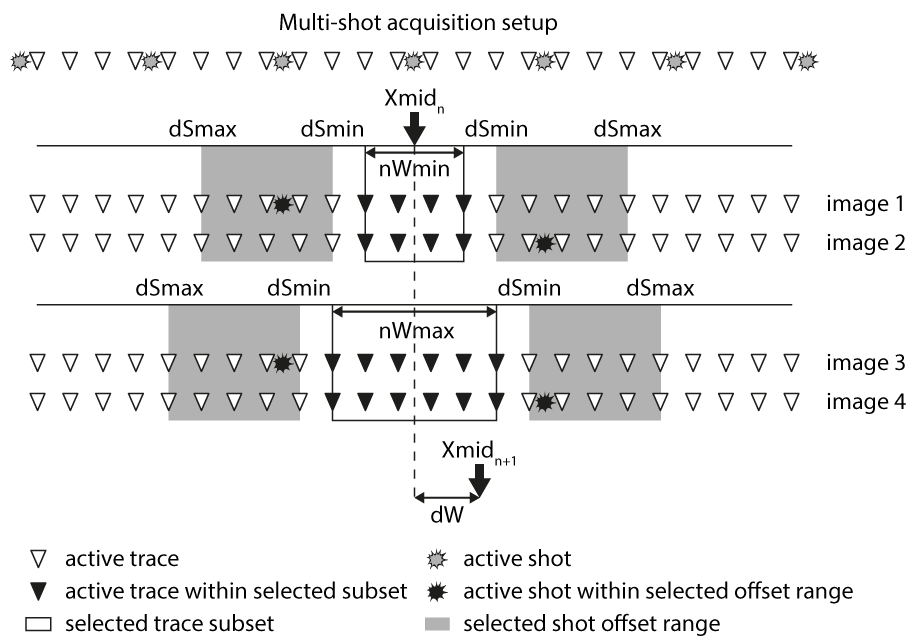
\includegraphics[width=0.75\linewidth]{figures/stack_wind.png}}
\caption{Stacking and windowing workflow.}
\label{fig:stack_wind}
\end{figure}

\paragraph{P-omega transform settings (used if calc=1)}
\begin{itemize}
\setlength\itemsep{2ex}
\setlength{\parindent}{5ex}

\item Set the frequency range for dispersion image computation ($p-\omega$ stack) with \verb|fmin| and \verb|fmax|.

\item Define the number of phase velocity samples in the dispersion image with \verb|nray| and their range with \verb|vmin| and \verb|vmax|.

\item Define \verb|xsca| according to the format in wich your coordinates are saved in the SU file (e.g. \verb|xsca = 100| if your coordinates are saved in centimeters).
\end{itemize}

\paragraph{Filter and mute settings (used if calc=1)}
\begin{itemize}
\setlength\itemsep{2ex}
\setlength{\parindent}{5ex}

\item Set \verb|filt = 1| to apply a band pass filter to the seismic data before the $p-\omega$ stack, or \verb|filt = 0| otherwise.

\item Define the frequency limits of the filter \verb|fcutlow| and \verb|fcuthigh|, along with the apodisation parameter \verb|taper|.

\item Set \verb|mute = 1| to apply a mute\footnote{The mute consists in zeroing samples before and/or after a specific time.} to the seismic data before the $p-\omega$ stack, or \verb|mute = 0| otherwise.

\item Define the first and last trace upper mute limits with \verb|tmin1| and \verb|tmin2|, and the first and last trace lower mute limits with \verb|tmax1| and \verb|tmax2|.
\end{itemize}

\paragraph{Dispersion picking settings}
\begin{itemize}
\setlength\itemsep{2ex}
\setlength{\parindent}{5ex}

\item Set \verb|pick = 1| to manually pick dispersion curves. I recommend to first start the script with \verb|calc = 1| and \verb|pick = 0|, then once it's done restart it with \verb|calc = 0| and \verb|pick = 1| (picking while calculating can take a really long time). To use the automatic picking option (\verb|pick = 2|), you first need to pick one dispersion curve with \verb|pick = 1|. It will then look for dispersion maxima in the range of the first picked dispersion curve.

\item \verb|mappick| defines the colormap used for the picking. While picking, you will be able to change the colormap for a specific Xmid, but it will always start with \verb|mappick| for each new Xmid.

\item Set \verb|mappicklog = 1| to use a "logarithmic" colorscale, or \verb|mappicklog = 0| for a linear colorscale.

\item \verb|dvmin| is the minimum phase velocity sample (in m/s) used to display and pick the dispersion. This option is used to accelerate display when picking, but will reduce the resolution of the picked phase velocity dispersion curves, which can be critical when dealing with small velocity variations. It has no impact on the saved dispersion images.

\item \verb|modeinit| is the first mode that is picked (0 corresponding to the fundamental mode, 1 to the first higher mode, 2 to the second higher mode,...). While picking, you will be able to change the picked mode for a specific Xmid, but it will always start with \verb|modeinit| for each new Xmid.

\item Set \verb|pickstyle = 1| to use semi-automatic picking (look for the closest maxima around the pick), or \verb|pickstyle = 0| to use full manual picking. While picking, you will be able to change the picking style for a specific Xmid, but it will always start with \verb|pickstyle| for each new Xmid.

\item Set \verb|smoothpick = 1| to smooth the picks with a moving average filter, or \verb|smoothpick = 0| for no smoothing. While picking, you will be able to change the smoothing style for a specific Xmid, but it will always start with \verb|smoothpick| for each new Xmid.\\[2ex]
%
Picked dispersion curves are stored in subprojdir/file.pick. They are named according to the Xmid position and the corresponding mode (Xmid.Mmode.pvc), and contain three columns with the frequency, phase velocity and phase velocity error.\\[2ex]
%
During picking, the user can switch between Xmids and modes, add or delete points, save or discard the current picking, and change colormap, picking style and smoothing style (more details when running the script in the MATLAB Command Window). Saving new picks will results in the overwriting of previously picked dispersion curves.

\end{itemize}

\paragraph{Dispersion curves sampling settings}
\begin{itemize}
\setlength\itemsep{2ex}
\setlength{\parindent}{5ex}

\item Set \verb|target = 1| to convert picked dispersion curves into the target files required for the inversion software, or \verb|target = 0| otherwise.

\item Set \verb|wave = 'R'| to create Rayleigh waves target, or \verb|wave = 'L'| to create Love waves target.

\item \verb|maxmodeinv| corresponds to the maximum number of mode included in the target file (and that will be inverted). Leave empty to include all the picked modes.

\item Set \verb|sampling = 1| to resample the picked dispersion curves in wavelength, or \verb|sampling = 0| to resample the picked dispersion curves in frequency. A discretization in wavelength is generally recommended to invert depth consistent data and prevent from giving excessive weight to high frequency samples which correspond only to the shallowest part of the medium.

\item \verb|resampvec| is the vector along which dispersion curves are resampled. It has to be a wavelength vector (in m) if \verb|sampling = 1|, and a frequency vector (in Hz) if \verb|sampling = 0|.

\item Set \verb|freqlim = 0| to set manually the minimum frequency of the resampled dispersion curve, or \verb|freqlim = 1| to use an automatic cutoff frequency determined from an amplitude threshold on the spectrogram (cf. \verb|specampmin|).

\item \verb|fminpick| is the minimum frequency used to resample dispersion curves when \verb|freqlim = 0|. When \verb|freqlim = 1|, \verb|fminpick| will be the minimum automatic cutoff frequency allowed.

\item \verb|specampmin| is the minimum amplitude of the spectrogram (in normalized units) used to determine the automatic cutoff frequency.\\[2ex]
%
Target files are stored in subprojdir/file.targ and contain all modes selected for inversion. They are named according to their Xmid position (Xmid.target). If a target file already exists for the selected Xmid when using \verb|target = 1|, it will be overwritten. Run the script with \verb|calc = 0| and \verb|pick = 0| to change only the targets parameter (sampling, number of modes, error type,...).

\end{itemize}

\paragraph{Error settings (used if target=1)}
\begin{itemize}
\setlength\itemsep{2ex}
\setlength{\parindent}{5ex}

\item Set \verb|err = 1| to define a phase velocity empirical error depending on the frequency and the window size (Lorentz error), \verb|err = 2| to define a phase velocity percentage error, or \verb|err = 0| for no error.

\item \verb|nWfac| allows to tweak the Lorentz error in order to increase (\verb|nWfac < 1|) or reduce (\verb|nWfac > 1|) the size of the error bars by calculating the error as if the mean window size nW was actually nW*nWfac. It is used only if \verb|err = 1|.

\item \verb|minerrvel| is the minimum velocity error (in m/s) allowed when \verb|err = 1|. It prevents having too small error bars at high frequency in which no theoretical model could fit.

\item \verb|maxerrrat| is the maximum velocity error ratio allowed when \verb|err = 1|. It prevents having too big error bars at low frequency in which all theoretical models could fit.

\item \verb|sigma| is the percentage of the velocity used to define the error when \verb|err = 2|.

\end{itemize}

\paragraph{Plot settings}
\begin{itemize}
\setlength\itemsep{2ex}
\setlength{\parindent}{5ex}

\item Set \verb|plotdisp = 1| to plot and save stacked dispersion images in subprojdir/file.img/1D\_data/disp (\verb|plotdisp = 0| for no plot).

\item Set \verb|plotpckdisp = 1| to plot and save stacked dispersion images with picked dispersion curves in subprojdir/file.img/1D\_data/disp\_pick (\verb|plotpckdisp = 0| for no plot).

\item Set \verb|plotspec = 1| to plot and save stacked spectrograms in subprojdir/file.img/1D\_data/spectro (\verb|plotspec = 0| for no plot).

\item Set \verb|plotseismo = 1| to plot and save stacked seismograms in subprojdir/file.img/1D\_data/seismo (\verb|plotseismo = 0| for no plot).

\item Set \verb|plotsingle = 1| to plot and save single seismogram, spectrograms and dispersion images in subprojdir/file.img/1D\_data/prestack (\verb|plotsingle = 0| for no plot).

\item Set \verb|plotstkdisp = 1| to plot and save intermediate stacked dispersion images in subprojdir/file.img/1D\_data/synstack (\verb|plotstkdisp = 0| for no plot).

\item Set \verb|plot1dobs = 1| to plot and save dispersion curves in subprojdir/file.img (\verb|plot1dobs = 0| for no plot).

\item Set \verb|plot2dobs = 1| to plot and save phase velocity pseudo-section in subprojdir/file.img (\verb|plot2dobs = 0| for no plot).

\item Set \verb|showplot = 1| to display the plots on the screen (\verb|showplot = 0| for no display).
\end{itemize}



\subsubsection{Module B\_SWIPparam}

\subsubsection{Module C\_SWIPinv}

\subsubsection{Module D1\_SWIPmod1d}

\subsubsection{Module D2\_SWIPmod2d}

\subsection{List of SWIP options}

\subsection{List of SWIP functions}

\end{document}
